\documentclass{llncs}
\usepackage{llncsdoc}
\usepackage{amsmath}
\usepackage{amsfonts}
\usepackage{amssymb}
\usepackage{algpseudocode}
\usepackage{algorithm}
\usepackage{algorithmicx}
\usepackage{color}
\usepackage{gnuplottex}
\usepackage{graphicx}
\usepackage{subcaption}
\usepackage{microtype}
\usepackage[normalem]{ulem}
\captionsetup{compatibility=false}
\usepackage{tikz}
\usetikzlibrary{trees,automata,positioning}

%% For lattice figure
% Set the overall layout of the tree
\tikzstyle{level 1}=[level distance=3.0cm, sibling distance=1.3cm]
\tikzstyle{level 2}=[level distance=3.5cm, sibling distance=1.3cm]
\tikzstyle{level 3}=[level distance=3.5cm, sibling distance=1.3cm]

% Define styles for bags and leafs
\tikzstyle{l1} = [rectangle, text width=3em, text centered]
\tikzstyle{l2} = [rectangle, text width=5em, text centered]
\tikzstyle{l3} = [rectangle, text width=5em, text centered]

%\algloopdefx[IfContinue]{IfContinue}
%[1]{\textbf{if} #1 \textbf{then break}}

\algsetblockdefx[IfContinue]{IfContinue}{IfContinue}
{0}{0pt}
[0]{}
[1]{\textbf{if} #1 \textbf{then continue}}

\begin{document}
\section{On Patterns and Matrices}

%The very first objective of this paper is to generalize our ideas into a theoretic framework. Such a framework provides us with the necessary tools to formally define the problem and the idealized space of solutions. The VOUW framework consists of two parts: (1) a concise definition that allows us to reason about what one can and cannot expect to find from a set of data and what this data could look like, and (2) a generalized encoding scheme that connects our framework to the MDL-principle.
In this section we will introduce a method of describing and decomposing tabular or matrix-like data. It may look at bit formal to the reader at first, but it is actually a concise notation that allows us to reason about what one can and cannot expect to find from a set of data and what this data could look like. In later sections we will use these tools to gradually connect to the MDL-principle and finally to a practical implementation.

The concepts that we present here are defined on bounded, discrete and two-dimensional geometric data. We represent this data as an $M\times N$ matrix $A$ whose rows and columns are finite and in a fixed ordering (i.e. reordering rows and columns semantically alters the matrix). Elements $a_{i,j}$, where row $i$ is on $[0;N)$ and column $j$ is on $[0;M)$, are of the integral type and more specifically a finite subset of $\mathbb{N}$ which we will denote as $\mathbb{N}_A$. We will denote $A$ as a matrix because of the convenience of the linear algebra notation. In any practical application however, $A$ will not represent a system of linear equations but rather hold some form of sampled data that can be places on a grid.

%\sout{A prerequisite is that a probability distribution $P_A$ is defined on the elements of $\mathbb{N}_A$, as we will need it later for encoding the elements of $A$. As for real-world data it is feasible to create a probability mass function by counting the values of $A$ (for example, when loading the dataset), we will from now on assume that $P_A$ is always defined.}

Kolmogorov complexity tells us to search for the shortest program that generates $A$. Examining this program then tells us everying there is to know about $A$ in the most succinct way possible. Although it has been proven that Kolmogorov complexity cannot be computed and thus this `ideal' cannot be attained, it can be approached. The principle behind MDL is that we can approximate an optimal description through the compression of the original data. This essentially means that we will limit the language that can be used to describe $A$ with in such way that we have a better chance of computing the optimal (shortest) program or description. This optimal description, let us call it $A'$, is only optimal if we can unambiguously reconstruct $A$ from it and nothing more (i.e., `lossless compression'). Intuitively compression means that we would like to have a way to just define $A$ using as few building blocks as possible. We illustrate this using the example in Figure \ref{example1}. Given the matrix $A$ we try to decompose it in (possibly recurring) substructures we call the \emph{patterns}, denoted $X$ and $Y$ in the example. For every matrix $A$ we have a collection of all possible patterns which we call the \emph{model} of a $A$, denoted $H_A$. Given only these patterns, $A$ cannot be reconstructed because we need a mapping from the model $H_A$ back to $A$. This mapping represents in what MDL calls the \emph{matrix $A$ given the model $H_A$}. In statistics this is often the structural versus the accidental information, but in this context we think of it merely as `instructions' of how to reconstruct $A$. Let us call the set of all instructions required to rebuild $A$ from $H_A$ the \emph{instantiation} of $H_A$. It is denoted by $\bar{H}_A$ in the example. Notice how this instantiation essentially tells us where in $A$ each pattern from $H_A$ was originally located.  The result is a notation that allows us to express matrix $A$ as if decomposed into sets of local and global spatial information.

Now that we have this top-down concept of the decomposition of $A$, we will continue to describe its constituents in more detail.

%We call a specific set of patterns $H\in \mathcal{H}_A$ a \emph{point hypothesis} and analogously a specific instantiation is denoted $\bar{H} \in \bar{\mathcal{H}}_A$. Formally, a complete description $A'$ of $A$ is a combination of some $H$ and $\bar{H}$ such that $\bar{H}$ is a 1-to-1 mapping from $H_A$ to $A$. In the next sections we will formalize these concepts by starting bottom-up with patterns and instances up to models, instantiation matrices and their link with MDL. After this we will discuss how we propose to find a good description of $A$ by means of the VOUW algorithm.

\begin{figure}

\small
$$
A =
\begin{bmatrix}
1 & \cdot & \cdot & \cdot & \cdot & 1 &  \\[-.2em]
\cdot & 1 & \cdot & \cdot & \cdot & \cdot &  \\[-.2em]
1 & \cdot & \cdot & \cdot & 1 & \cdot &  \\[-.2em]
\cdot & 1 & \cdot & \cdot & \cdot & 1 &  \\[-.2em]
1 & \cdot & 1 & \cdot & \cdot & \cdot &  \\[-.2em]
\cdot & 1 & \cdot & 1 & \cdot & \cdot &  \\
\end{bmatrix}\!\!,
\bar{H} = 
\begin{bmatrix}
X & \cdot & \cdot & \cdot & \cdot & Y &  \\[-.2em]
\cdot & \cdot & \cdot & \cdot & \cdot & \cdot &  \\[-.2em]
X & \cdot & \cdot & \cdot & X & \cdot &  \\[-.2em]
\cdot & \cdot & \cdot & \cdot & \cdot & \cdot &  \\[-.2em]
X & \cdot & X & \cdot & \cdot & \cdot &  \\[-.2em]
\cdot & \cdot & \cdot & \cdot & \cdot & \cdot &  \\
\end{bmatrix}\!\!,
H = \{
X =
\begin{bmatrix}
1 & \cdot \\[-.2em]
\cdot & 1
\end{bmatrix}\!\!,
Y =
\begin{bmatrix}
1
\end{bmatrix}\}
$$
\caption{Example decomposition of $A$ into instantiation $\bar{H}$ and patterns $X,Y$}
\label{example1}
\end{figure}

\subsection{Patterns and Instances}
Intuitively we can think of a pattern as some submatrix $B$ of the original matrix $A$. This submatrix is not necessarily complete (elements may be $\cdot$), which gives us the ability to precisely cut-out any irregular-shaped part of $A$. We additionally require the elements $B$ to be adjacent (horizontal, vertical or diagonal) to at least one non-empty element. While this limits the amount of possible patterns somewhat, it will later on also reduce the computational effort dramatically. We will now define a pattern to be the smallest submatrix to completely contain all elements of $B$.

\begin{definition}
We define \textbf{pattern} $X$ as an $M_X\times N_X$ submatrix of $A$ where any non-empty element may optionally be replaced by $\cdot$ such that:
\begin{itemize}
\item Any non-empty element in $X$ is adjacent (horizontal, vertical or diagonal) to at least one other non-empty element.
\item The first and last rows and columns contain at least one non-empty element.
\end{itemize}
\end{definition}

From this definition we see that the dimensions $M_X\times N_X$ give essentially the smallest rectangle around $X$ (the \emph{bounding box}. As a more useful measure we therefore also define the cardinality $|X|$ of $X$ as the number of non-empty elements. We call pattern $X$ with $|X|=1$ a \emph{singleton pattern}, i.e. a pattern containing exactly one element of $A$. Furthermore we will often slightly abuse notation by using single-index elements or using set notation for any matrix. For instance, when we write $x_i \in X$, we mean that $x_i$ is the $i$-th non-empty element in $X$ with $1\leq i \leq |X|$. By convention we will always use row-major ordering in these cases.

One element in each pattern is given the special function of \emph{pivot}. 

\begin{definition}
The \textbf{pivot} $p(X)$ of pattern $X$ is the first non-empty element of $X$ in the first non-empty column of the first (non-empty) row of $X$.
\end{definition}

A pivot can be thought of as a fixed point in a pattern $X$ which we can use to position its elements in relation to $A$. The precise translation we apply to a particular pattern we call an \emph{offset}. An offset is a tuple $\delta=(i,j)$ that is on the same domain as an index in $A$. We realize this translation by placing all elements of $X$ on an empty $M\times X$ size matrix in such way that the pivot element is at $(i,j)$. We formalize this concept with the \textbf{instantiation operator} $\oplus$ .

\begin{definition}
In the context of an $M\times N$ matrix $A$, we define the \textbf{instance} $X \oplus \delta$ as the incomplete $M\times N$ matrix containing all elements of $X$ such that the pivot $p(X)$ is at index $(i,j)$ and the distances between all original elements are preserved. The resulting matrix contains no additional non-empty elements. 
\end{definition}

So according to this definition $\oplus$ adds `padding' around the elements a pattern to align its pivot to a certain offset $(i,j)$. Obviously this does not yield a valid result for an arbitrary offset $(i,j)$. We want to limit ourselves to the space of pattern instances that are actually valid in relation to matrix $A$. Therefore two simple constraints are needed: (1) an instance must be \emph{well-defined}: placing pivot $p(X)$ is at index $(i,j)$ results in a $M\times N$ matrix that contains all elements of $X$. Furthermore, (2) elements of instances cannot overlap, meaning each index of $A$ should be described at most once. This ensures the description is both unambiguous and minimal.

\begin{definition}
Two pattern instances $X \oplus \delta_x$ and $Y \oplus \delta_y$, with $\delta_x \neq \delta_y$ are \textbf{non-overlapping} if $|(X \oplus \delta_x) + (Y \oplus \delta_y)| = |X|+|Y|$.
\end{definition}

The definitions for patterns and their instances now give the appropriate tools to describe a mapping from sets of patterns to the original matrix $A$. Say we have a set of patterns $H$ over $A$, we would like to have a set of `instructions' of where instances of each pattern should be positioned in order to obtain $A$. When we look at the example in Figure \ref{example1}, we see that we could use again a $M\times N$ matrix for this. This matrix contains elements that are in $H$ such that each index corresponds to the offset of that specific pattern's instance.

\begin{definition}
Given the set of patterns $H$, the \textbf{instantiation (matrix)} $\bar{H}$ is an incomplete $M\times N$ matrix with the set of possible elements being $H$, i.e. $\bar{h}_{i,j} \in H$ for all $(i,j)$. For all non-empty elements $\bar{h}_{i,j}$ it holds that $\bar{h}_{i,j} \oplus (i,j)$ is an instance of $\bar{h}_{i,j}$ in $A$ that is not non-overlapping with any other instance $\bar{h}_{i',j'} \oplus (i',j')$.
\end{definition}

The above definition does the interesting proposition that the offset to each instance is unique. Given that a pattern's pivot is placed exactly at one offset and that instances must be non-overlapping, makes this indeed believable. Later when we inductively define the set $\bar{H}$ of all instantiation matrices, this will be shown to be true more formally. 

\subsection{Constructing Patterns [verplaatsen naar H2]}

As patterns are the building blocks of our model we also need to have a practical way to construct them. We will do this by joining smaller patterns together to create increasingly large patterns and, as we will later see, this concept also forms the basis of the search algorithm. However, two patterns could be joined in any different number of ways. We can define the exact way two patterns should be joined by enumerating the distance of their respective pivot. In order to this we, we use pattern instances as an intermediate step.

Recall that instances are simply patterns projected on an $M\times N$ matrix, containing the same elements as the pattern at their original distances. This makes $\oplus$ trivially reversible by removing all completely empty rows and columns.

\begin{definition}
Let $X \oplus \delta$ be an instance of $X$, then by definition we say that $\ominus(X \oplus \delta) = X$.
\end{definition}

We can now define a sum on two instances to get a new instance that combines both operands. Even though the result is not a pattern, we can always obtain it by using $\ominus$. The example in Figure \ref{example2} illustrates this process. We start by instantiating $X$ and $Y$ with offsets $(1,0)$ and $(1,1)$ respectively. This yields the non-overlapping $\bar{X}$ and $\bar{Y}$, which we simply add up to obtain $\bar{Z}$. The new pattern contained in $\bar{Z}$ can be easily identified by removing the top empty row. We formally describe this mechanism in Theorem \ref{fundamental}. As we will see later, this is the fundamental operation of the algorithm.

\begin{figure}

\small
$$
X =
\begin{bmatrix}
1 & \cdot \\[-.2em]
\cdot & 1
\end{bmatrix}\!\!,
Y =
\begin{bmatrix}
1
\end{bmatrix}\!\!,
\bar{X} = X\oplus (1,0) =
\begin{bmatrix}
\cdot & \cdot \\[-.2em]
1 & \cdot \\[-.2em]
\cdot & 1
\end{bmatrix}\!\!,
Y\oplus (1,1) =
\begin{bmatrix}
\cdot & \cdot \\[-.2em]
\cdot & 1 \\[-.2em]
\cdot & \cdot
\end{bmatrix}\!\!,
\bar{X} + \bar{Y} =
\begin{bmatrix}
\cdot & \cdot \\[-.2em]
1 & 1 \\[-.2em]
\cdot & 1
\end{bmatrix}\!\!,
Z =
\begin{bmatrix}
1 & 1 \\[-.2em]
\cdot & 1
\end{bmatrix}\!\!
$$
\caption{Example of Theorem \ref{fundamental}. The $2\times 3$ input matrix is not shown.}
\label{example2}
\end{figure}

\begin{theorem}\label{fundamental}
Given two non-overlapping instances $\bar{X}=X\oplus \delta_X$ and $\bar{Y}=Y\oplus \delta_Y$, the sum of the matrices $\bar{X} + \bar{Y}$ is another instance. We observe that pattern $Z=\ominus(\bar{X} + \bar{Y})$ such that $\bar{X} + \bar{Y} = Z\oplus \delta_X$.
\end{theorem}

Notice that this sum has the limitation that two instances can only be summed if they do not overlap. While this is a serious limitation, we will show in the next section that it is not of any practical relevance.

\subsection{Structural Equivalence}

In the previous sections we silently omitted an important constraint in instantiating patterns. An instance has only meaning in the context of matrix $A$ if their respective elements match. In order words, if an instance $X \oplus (i,j)$ has all its non-empty elements identical to the corresponding indices in $A$, this means that pattern $X$ matches $A$ in $(i,j)$. In this case the match is exact, formally
\begin{definition}
The instance $\bar{X}=X \oplus \delta$ is an \textbf{exact match on $A$} if for all non-empty $\bar{x}_{i,j} \in \bar{X}$ holds that $\bar{x}_{i,j} = a_{i,j}$.
\end{definition}

While this form of straightforward matching can be desirable in some cases, it may lead to a bloated model in others. Take the example from Figure \ref{example3} that lists matrix $A$ and four patterns. Pattern $W$ is obviously an exact match to five of the six elements of $A$. Pattern $X$, while not an exact match, is also a good candidate to describe $A$ although it is multiplied by a constant factor of two. Pattern $Y$ is a near-exact match: only one element is off - this could be due to noise for example. Pattern $Z$ is no match for the values in $A$, but notice that it is identical in structure to the other patterns: it places as many values at the same indices. 

\begin{figure}
\small
$$
\left.
A =
\begin{bmatrix}
1 & 2 \\[-.2em]
\cdot & 1 \\[-.2em]
1 & 2
\end{bmatrix}\
\right\rvert
W =
\begin{bmatrix}
1 & 2 \\[-.2em]
\cdot & 1 \\[-.2em]
1 & 2
\end{bmatrix}\!\!,
X =
\begin{bmatrix}
2 & 4 \\[-.2em]
\cdot & 2 \\[-.2em]
2 & 4
\end{bmatrix}\!\!,
Y =
\begin{bmatrix}
1 & 2 \\[-.2em]
\cdot & 1 \\[-.2em]
1 & 1
\end{bmatrix}\!\!,
Z =
\begin{bmatrix}
2 & 2 \\[-.2em]
\cdot & 0 \\[-.2em]
4 & 3
\end{bmatrix}\!\!,
$$
\caption{Examples of structurally equivalent patterns with varying degrees of similarity.}
\label{example3}
\end{figure}

The example above suggest that we could do one more step of decomposition: just like we decomposed the original matrix into global structure (instantiation) and local structure (pattern), we decompose patterns into structure and magnitude. 

\begin{definition}
The \textbf{structure matrix} $S(X)$ of pattern $X$ is an equally-sized boolean matrix such that $S(X)_{i,j}=1$ whenever $X_{i,j}$ is non-empty.\\
The \textbf{magnitude} $M(X)$ of pattern $X$ is the string of values obtained by taking each non-empty element of $X$ in row-major order.
\end{definition}

In the example we can see that $S(X)= \tiny\begin{bmatrix}1 & 1 \\[-.2em]\cdot & 1 \\[-.2em]1 & 1\end{bmatrix}$ and that $M(X)=1\ 2\ 1\ 1\ 2$. In fact, because all four patterns have the same structure matrix, we say that they are \emph{structurally equivalent}. As such we write $X \cong Y$ iff $S(X) = S(Y)$. 

To understand the importance of separating the structure and magnitude of patterns, let us briefly expand the example above. Suppose we have a large matrix $B$ that consists out of $n$ clusters of matrices $W$ and $X$ from Figure \ref{example3}. To determine the optimal description of $B$, we might want to look at the prevalence of each submatrix. Say it contains $\frac{n}{2}$ $W$'s and $\frac{n}{2}$ $X$'s. In this case it makes sense to include both patterns in the description. However, we could also exploit the fact that the structure of both patterns is equivalent and make the description more concise by only storing $S(W)$ and then $M(W)$ and $M(X)$ separately. Now imagine that $B$ only contains one $W$ and $n-1$ $X$'s. In this case the one $W$ might be an anomaly that we would like to detect. However, it could also be due to noise in the data in which case we would like to describe $B$ just using $n$ $X$'s. It is impossible to make this distinction beforehand. 

One possibility for solving this problem is to let Kolmogorov complexity decide whether the stray $W$ is an anomaly or not. Recall that according to Kolmogorov complexity the most succinct description is the best. Therefore if the amount of `effort' required to transform $X$ into $W$ is small, we should probably encode that one $W$ using $X$. In that case it is considered noise, while it is probably an anomaly if doing so would yield a larger description.


\section{The Problem and its Solution Space}
%\subsection{The Set $\mathcal{H}_A$ and $\bar{\mathcal{H}}_A$}\label{thesetH}

In the previous section we have given a means to describe a matrix $A$ in a different way, namely that of patterns and instances. If we succeed in describing $A$ in our notation in a more concise way than just $A$ itself, we have learned something about the local and global structure of $A$ and perhaps even about anomalies or noisy values. Here the relation between Kolmogorov-complexity and learning is quite clear. In order to find this shortest description, however, we will first have to define our search space and the way solutions are to be constructed.

We begin by defining the \emph{model class} $\mathcal{H}$, the set of all possible models for all possible inputs. Without any prior knowledge, this is the search space of our algorithm. A more bounded subset of $\mathcal{H}$ is the the set of all possible models for $A$ and the set of all possible instantiations to these models. We will write these sets as $\mathcal{H}_A$ and $\bar{\mathcal{H}}_A$ respectively, and describe them first. To this end will first take $H_A^0$ to be the model with only singleton patterns (patterns of length 1). As singletons are just individual elements of $A$, we can simply say that $H_A^0=\mathbb{N}_A$. The instantiation matrix to $H_A^0$ is denoted $\bar{H}_A^0$. Given that each element of this matrix must correspond to exactly one element of $A$ in $H_A^0$, we see that each $\bar{h}_{i,j} = a_{i,j}$ and so $\bar{H}_A^0$ is equal to $A$. 

Using $H_A^0$ and $\bar{H}_A^0$ as base cases we can now inductively define the set $\bar{\mathcal{H}}_A$ of all instantiations of all models over $A$:\\
\textbf{Base case:} $\bar{H}_A^0 \in \bar{\mathcal{H}}_A$\\
\textbf{By induction:} If $\bar{H}$ is in $\bar{\mathcal{H}}_A$ then take any pair $\bar{h}_{i,j},\bar{h}_{k,l} \in \bar{H}$ such that $(i,j)\leq(k,l)$ in lexicographical order. The set $\bar{H}'$ is also in $\bar{\mathcal{H}}_A$ for $\bar{H}' = \bar{H}$ and
\begin{align*}
\bar{h}_{i,j}' &:= \ominus \big( \bar{h}_{i,j} \oplus (i,j) + \bar{h}_{k,l} \oplus (k,l) \big) \\
\bar{h}_{k,l}' &:= \cdot
\end{align*}

In this definition of $\bar{H}_A^0$ we inductively replace two instances with their sum. Indeed we can add any two instances together in any order and eventually this results in just one big instance that is equal to $A$. The elegance in this is that by this inductive definition, the instances never overlap and thus their sum is always a valid instance on $A$. Note that when we take two elements $\bar{h}_{i,j},\bar{h}_{k,l} \in \bar{H}$ we force $(i,j)\leq(k,l)$ to be in lexicographical order, we know the pivot of the new pattern to coincide with $\bar{h}_{i,j}$, since the pivot is the first element in lexicographical order. We can then leave $\bar{h}_{k,l}$ empty.

The construction of instantiation matrices also implicitly defines the corresponding models. While this may seem odd - defining models for instantiations instead of the other way around - note that there is no unambiguous way to find an instantiation matrix for a given model. Instead we find the following trivial definition by applying the inductive construction rule above.
\begin{definition}
The set $\mathcal{H}_A$ of all models over $A$ is the set such that 
$$
\mathcal{H}_A=\Big\{\big\{\ominus(\bar{h}_{i}) \ | \ i \in \{1\dots |\bar{H}|\}\big\} \ \Big | \ \bar{H} \in \bar{\mathcal{H}}_A \Big\}.
$$ 
\end{definition}
So for any instantiation $\bar{H}\in \bar{\mathcal{H}}_A$ there is a corresponding set in $\mathcal{H}_A$ of all patterns that occur in $\bar{H}$. This results in an interesting symbiosis between model and instantiation: increasing the complexity of one decreases that of the other. When plotting this construction a tightly connected lattice appears such as that of Figure \ref{lattice}. 
%\begin{theorem}
%Given any instantiation $\bar{H}\in \bar{\mathcal{H}}_A$ and its corresponding model in $%\mathcal{H}_A$, the matrix $A$ can be reconstructed unambiguously.
%\end{theorem}

\begin{figure}
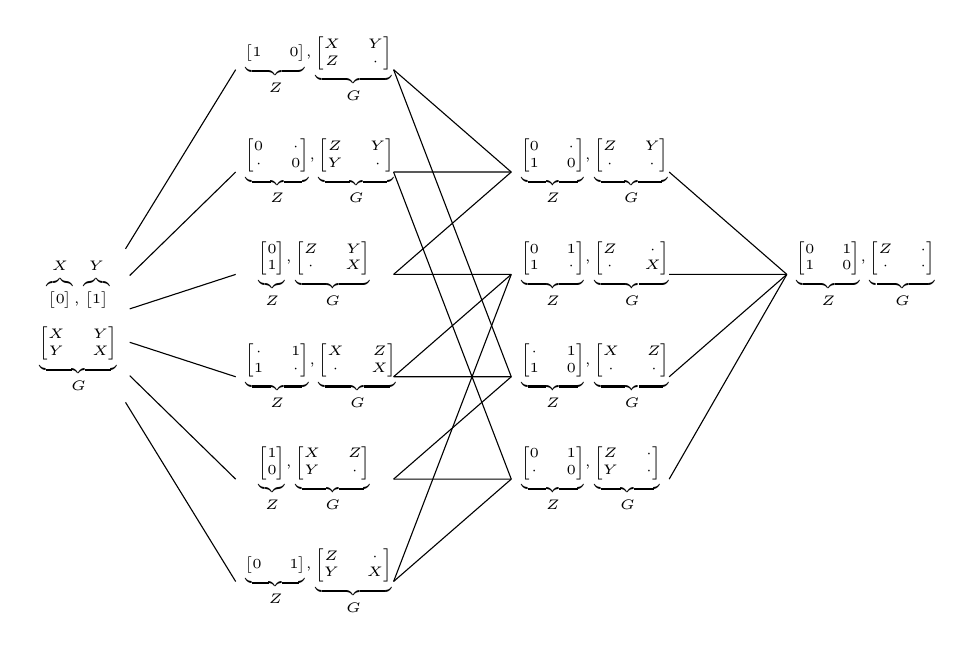
\begin{tikzpicture}[on grid, grow=right]
\node(R)[l1] {\tiny $\begin{matrix}\overbrace{\begin{bmatrix}0\end{bmatrix}}^{X},\overbrace{\begin{bmatrix}1\end{bmatrix}}^{Y}\\[1em]\underbrace{\begin{bmatrix}X & Y \\Y & X\end{bmatrix}}_{G}\end{matrix}$}
	child {
        node(F)[l2] {\tiny $\underbrace{\begin{bmatrix}0 & 1\end{bmatrix}}_{Z},\underbrace{\begin{bmatrix}Z & \cdot \\Y & X\end{bmatrix}}_{G}$}        
            edge from parent[draw=none] 
            (R) edge (F.west)
    }
    child {
        node(E)[l2] {\tiny $\underbrace{\begin{bmatrix}1 \\ 0\end{bmatrix}}_{Z},\underbrace{\begin{bmatrix}X & Z \\ Y & \cdot\end{bmatrix}}_{G}$}        
            child {
                node(J)[l3]
                    {\tiny $\underbrace{\begin{bmatrix}0 & 1 \\ \cdot & 0\end{bmatrix}}_{Z},\underbrace{\begin{bmatrix}Z & \cdot \\ Y & \cdot\end{bmatrix}}_{G}$}
                edge from parent 
            }
            edge from parent[draw=none] 
            (R) edge (E.west)
    }    
    child {
        node(D)[l2] {\tiny $\underbrace{\begin{bmatrix}\cdot & 1 \\ 1 & \cdot\end{bmatrix}}_{Z},\underbrace{\begin{bmatrix}X & Z \\ \cdot & X\end{bmatrix}}_{G}$}        
            child {
                node(I)[l3]
                    {\tiny $\underbrace{\begin{bmatrix}\cdot & 1 \\ 1 & 0\end{bmatrix}}_{Z},\underbrace{\begin{bmatrix}X & Z \\ \cdot & \cdot\end{bmatrix}}_{G}$}
                edge from parent 
            }
            edge from parent[draw=none] 
            (R) edge (D.west)
    }    
    child {
        node(C)[l2] {\tiny $\underbrace{\begin{bmatrix}0 \\ 1\end{bmatrix}}_{Z},\underbrace{\begin{bmatrix}Z & Y \\\cdot & X\end{bmatrix}}_{G}$}        
            child {
                node(H)[l3]
                    {\tiny $\underbrace{\begin{bmatrix}0 & 1 \\ 1 & \cdot\end{bmatrix}}_{Z},\underbrace{\begin{bmatrix}Z & \cdot \\ \cdot & X\end{bmatrix}}_{G}$
                    }                    
                    	child {
                    		node(K)[l3] {\tiny $\underbrace{\begin{bmatrix}0 & 1 \\ 1 & 0\end{bmatrix}}_{Z},\underbrace{\begin{bmatrix}Z & \cdot \\ \cdot & \cdot\end{bmatrix}}_{G}$}
                    	}
                edge from parent 
            }
            edge from parent[draw=none] 
            (R) edge (C.west)
    }    
    child {
        node(B)[l2] {\tiny $\underbrace{\begin{bmatrix}0 & \cdot \\ \cdot & 0\end{bmatrix}}_{Z},\underbrace{\begin{bmatrix}Z & Y \\Y & \cdot\end{bmatrix}}_{G}$}        
            child {
                node(G)[l3]
                    {\tiny $\underbrace{\begin{bmatrix}0 & \cdot \\ 1 & 0\end{bmatrix}}_{Z},\underbrace{\begin{bmatrix}Z & Y \\ \cdot & \cdot\end{bmatrix}}_{G}$}
                edge from parent 
            }
            edge from parent[draw=none] 
            (R) edge (B.west)
    } 
    child {
        node(A)[l2] {\tiny $\underbrace{\begin{bmatrix}1 &0\end{bmatrix}}_{Z},\underbrace{\begin{bmatrix}X & Y \\Z & \cdot\end{bmatrix}}_{G}$}        
        	edge from parent[draw=none] 
            (R) edge (A.west)
    };
\draw(F.east)--(H.west);
\draw(F.east)--(J.west);
\draw(B.east)--(J.west);
\draw(C.east)--(G.west);
\draw(D.east)--(H.west);
\draw(E.east)--(I.west);
\draw(A.east)--(G.west);
\draw(A.east)--(I.west);
\draw(G.east)--(K.west);
\draw(I.east)--(K.west);
\draw(J.east)--(K.west);
\end{tikzpicture}
\caption{The model space lattice for a $2\times 2$ binary matrix.}
\label{lattice}
\end{figure}

\subsection{The Optimal Model}

We have now found \emph{all} possible models for $A$ and have defined a nice method to construct both instance sets and models inductively. While this is certainly useful, we still need to find \emph{the optimal} model out of all these models. To this end we make the connection with the MDL-principle that says, informally, that the most concise encoding of the data gives us the best description. In this context that means the total size of $A'$, consisting of a model $H_A$ and an instantiation $\bar{H}_A$, must be minimized. We do this according to the two-part MDL equation, that seeks to minimize the sum of these two components:
$$
L_1(H_A) + L_2(A|H_A)
$$
Here the functions $L_1, L_2$ are two independent length functions that make up the coding scheme for two-part MDL. This minimization is often thought of as compression, although we will not actually write any encoded data. This leaves is with the task of finding an encoding scheme that encodes both model and instantiations lossless and without redundancy.

Say we have some set of symbols $S=\{S_0,S_1,\dots,S_n\}$ and each symbol has a length $l_0,l_1,\dots,l_n$. These symbols could be for example be a code word for each pattern $X_0, X_1,\dots,X_n$ in a model. We now want to find lengths $l_i$ using the Kraft-inequality such that holds that $\displaystyle\sum^N_{i=0}r^{-l_i} \leq 1$. In this case we say that $r=2$, because there are two symbols (0 and 1) in our code alphabet so we can measure code lengths in bits. 
The Kraft-inequality gives us a bijection between code lengths and probability distributions. This is one of the main ideas of the MDL-principle. So in our example we can write a probability distribution $P(X), X \in H_A$ as the chance of pattern $X$ occurring in our instance set. Given these probabilities we can use Shannon's Entropy $l_i=-\log(P(X_i))$ to compute the exact number of bits a pattern should optimally be encoded with.

Notice how common code words are shorter then rarely used code words. According to the Kraft-inequality this gives us an optimal code. The number of bits we compute are real numbers and not integers. While this does certainly not result in a practical encoding, we do not actually need to encode the data as we are only interested in its hypothetical length.

\subsection{Encoding Models and Instantiations}
To be able to compute the length of a given code word we must know the probability of that word occurring in our data. This information must also be available to the hypothetical decoder as otherwise the encoding is not lossless. Sometimes this is not practical as we do not know the probability distribution beforehand. For example, given an arbitrary encoded $A'$, we do not know the probability that each pattern occurs in the instantiation matrix. Although we could also encode this information separately, it would only incur an undue bias.

Fortunately we can still encode information without knowing or encoding the probabilities. One coding we will use is the universal code integers \cite{integerprior}. The corresponding length function $L_{\mathbb{N}}(n)$ gives the number of bits required to encode and arbitrary $n$ and is defined as $L_{\mathbb{N}}(n) = \log*(n) + \log(c_0)$ with $\log*(n) = \log(n) + \log \log(n) + \cdots$ and $c_0=2.865064$ to satisfy the Kraft-inequality. This code is obviously not uniform and assigns a longer code to a larger $n$. We will use this code to encode arbitrary integers.

To encode the instantiation matrix we will use \emph{prequential plug-in code} \cite{ppcode} instead. The prequential plug-in code is defined for sequences of one item at a time and updates the probability of each item as it is encoded, such that the probability need not be known in advance. It has the favourable property of being asymptotically equal to the optimal code for large sequences. Say we want to encode all elements $\bar{h}_i \in \bar{H}$ lexicographical order, we define:
\begin{definition}\label{plugin}
$$
P_{plugin}( y_i = \bar{h}_i \mid y^{i-1} ) = \frac{|\{y \in y^{i-1} \mid y = \bar{h}_i\}| + \epsilon }{\sum_{X \in H}|\{y \in y^{i-1} \mid y = X\}| + \epsilon}
$$
\end{definition}
Here $y_i$ is the i-th element to be encoded and $y^{i-1}$ is the sequence of elements encoded so far. We initialize the base case (no element has been sent yet) with a pseudocount $\epsilon$, which gives $P_{plugin}( y_1 = \bar{h} \mid y^{0} ) = \frac{\epsilon}{\epsilon|H|}$. We pick $\epsilon=0.5$ as it is used generally with good results.

In this case we do know the distribution as the encoder, but not as the decoder. This information can be used to slightly rephrase the definition above to be able to encode items in arbitrary order. The first step here is to determine the probability that each unique element (pattern) in $\bar{H}$ occurs. 

\begin{definition}\label{usage}
Given a set of instantiations $\bar{H}$, we define $U(X)$ as the \textbf{usage} of pattern $X$ such that
$$
	U(X) = |\{ \bar{h}_i \in \bar{H} \mid \bar{h}_i = X\}|.
$$
\end{definition}


From this definition we see that the \emph{usage} of a pattern is sum a of how often it occurs as an instance. Using this function we can rewrite Definition \ref{plugin} to produce the length of the instantiation matrix $\bar{H}$ as
\begin{align*}
	L_{pp}(\bar{H}\mid P_{plugin}) &= \sum^{|\bar{H}|}_{i=1} -\log \frac{|\{y \in y^{i-1} \mid y = \bar{h}_i\}| + \epsilon }{\sum_{X \in H}|\{y \in y^{i-1} \mid y = X\}| + \epsilon}\\
	&= \sum^{|H|}_{X_i \in h} -\log \prod^{U(X_i)-1}_{j=0} \frac{j+\epsilon}{\sum^{i-1}_{k=1} U(X_k)+j+\epsilon|H|} \\
	&= -\log \frac{\prod^{X_i\in H} \prod^{U(X_i)}_{j=0} j + \epsilon}{\prod^{|\bar{H}|-1}_{j=0} j + \epsilon|H|} \\
	&= -\sum^{|H|}_{X_i \in h} \left[ \log \frac{\Gamma(U(X_i)+\epsilon)}{\Gamma(\epsilon)}\right] + \log \frac{\Gamma(|\bar{H}| + \epsilon|H|)}{\Gamma(\epsilon|H|)}
\end{align*}

Here we use the fact that we can interchange sums of logarithms with logarithms of products and that those terms can be moved around freely. Moreover we convert the real-valued product sequences to the Gamma function $\Gamma$, which is the factorial function extended to real and complex numbers such that $\Gamma(n) = (n-1)!$.

Lastly, in addition to $L_{\mathbb{N}}$ and $L_{pp}$ we also define the length of the uniform distribution $L_0(n)=log(n)$. That is, when $n$ items have equal probability they all receive a code of equal length $log(n)$.

\subsubsection{The length function for incomplete matrices.}

To losslessly encode $A'$ we have to encode both $H$ and $\bar{H}$ individually. Recall that both instantiations and patterns are both matrices. For this we are in the unique position to use the same encoding for both the model and the `data given the model'. The only difference is that the probability distributions differ: for patterns we know the distribution of elements in $A$ to be $P_A$ beforehand while for the instantiation matrix we use the prequential coding.

\begin{definition} We define $L_{mat}( X | P )$ as the length function on $M\times N$ matrix $X$ given a probability function $P$ on elements of $X$ to be
$$
	L_{mat}( X | P ) = L_{\mathbb{N}}(M) + L_{\mathbb{N}}(N) + L_0(MN) + L_{\mathbb{N}}(\binom{MN}{|X|}) + \sum_{x_i \in X} -\log P(x_i)
$$
\end{definition}

TODO: conclude and perhaps define gain() here and move prequential coding part here?

\section{The VOUW Algorithm}

Now that we have finalized the theoretical foundation we can begin to formulate the problem and work towards an algorithmic solution. Before we do so, however, we take a moment to sketch the complexity of the current solution space. In order to do this we use the same steps as the inductive definition of $\bar{\mathcal{H}}_A$ as given in section \ref{thesetH}. We start with $\bar{H}=\bar{H}_A^0$, which by definition contains exactly $MN$ instances. We then pick two arbitrary instances and replace these with their sum to obtain $\bar{h}'$. Simple combinatorics say we can do this in $\binom{MN}{2}$ ways. Since now $|\bar{H}'| = MN-1$, we have $\binom{MN-1}{2}$ possibilities for the next step, and so forth until we have only one big instance left that contains exactly $A$ (the completely overfit model). We can simplify this sequence to
\begin{align}
\displaystyle\prod^{MN-2}_{n=0} \binom{MN-n}{2} = \displaystyle\prod^{MN-2}_{n=0} \frac{MN-n}{2(MN-n-2)!} = \frac{(MN)!(MN-1)!}{2^{MN-1}} .
\end{align}
While we must stress that this is an upper bound in the worst case that no pattern ever occurs more than once, the complexity class this naive approach yields is still quite impossible. In the remainder of the section we will describe a baseline algorithm that utilizes heuristics and additional constraints to reduce this complexity to close to linear.

\subsection{Heuristics}

It appears that it is not feasible to search the entire solution space due to the combinatorial explosion we have just seen. We will now describe a practical baseline algorithm that can search the solution space in close to linear time, if we are willing to find `a good solution' rather than `the optimal solution'. The baseline algorithm can be used to show complexity and give guarantees on convergence, while we will later modify it for practical applications by adding decomposition (a form of pruning) and support for domain-specific equivalence.

The first step is to add two additional constraints to the search:
\begin{enumerate}
\item The search must be \textbf{greedy}: when we unite two instances, we will never go back to a state where they are separate.
\item Two instances can only be united if they are \textbf{adjacent}.
\end{enumerate}

The first constraint is very straightforward. The greedy approach reduces the complexity considerably with the danger of converging on local minima. While this sounds problematic, notice that the discussed models are already an approximation. Therefore it is hard to justify the computational expenses looking for `the optimal approximation'. Furthermore, we will introduce an additional method later on that decreases the probability of convergence on local minima.

For the second constraint we must first define what we mean by \emph{adjacency}.
\begin{definition}
Two instances $\bar{x}_{i,j},\bar{x}_{k,l}\in \bar{H}$ are \textbf{adjacent} if
$$
	(i,j) < (k,l) \land l-j \leq \mathtt{colMax}(\ominus(\bar{x}_{i,j}))+1 \land l-j \geq \mathtt{colMin}(\ominus(\bar{x}_{i,j}))-1 \land k-i \leq \mathtt{rowMax}(\ominus(\bar{x}_{i,j}))+1.
$$
TODO: make more comprehensible, define colMax etc.
\end{definition}

Firstly we demand that the second instance comes after the first in lexicographical order. This is the same requirement as for the inductive definition of $\bar{\mathcal{H}}_a$ in Section \ref{thesetH}. We define the function $\mathtt{adjacent}(\bar{x})$ to be set of all instances adjacent to $\bar{x}$. Figure \ref{fig:adjacency} depicts more clearly what such a set looks like.

In order to compute complexity later, we would like to know the size of this set of adjacent instances. Fortunately it is trivial to give an upper bound for some instance $R=(X,t,\vec{p})$.
\begin{align}
	|\mathtt{adjacent}(\bar{x})| = \big(M_X+1\big) \times \big(N_X+1\big) - |X| + 1
\end{align}
Where $X=\ominus(\bar{x})$. According to this, the smallest possible instance whose image is a single element in $A$ has at most 4 adjacent instances. For the rest where complexity is concerned, we only need to know that the number of adjacent instances is on average roughly $O(|X|^{1.3})$.

\subsection{The baseline algorithm}

Now that we have defined and motivated the heuristics we use, it is time to discuss the algorithm itself. We will with an outline given by Listing \ref{alg:vouw}.

\begin{algorithm}
\caption{vouw}
\label{alg:vouw}
\begin{algorithmic}
\State $H \gets H_A^0$
\State $\bar{H} \gets \bar{H}_A^0$
\Repeat
	\State $C \gets \emptyset$ 
		\Comment Set of candidates
	\State $\forall_{c\in C} \ {usage}(c) = 0$
		\Comment Relation $C \to \mathbb{Z}$ stores occurrence per candidate
	\ForAll{$x_i \in \bar{H}$}
		\Comment i-th non-empty element in the instantiation matrix
		\ForAll{$\bar{y} \in \mathtt{adjacent}(\bar{x}_i)$}
		\State $X \gets \ominus(\bar{x}_i), \ Y \gets \ominus(\bar{y})$
		\State $\delta \gets {index}(\bar{y}) - {index}(\bar{y})$
		\State $c \gets (X,Y,\delta)$
			\Comment Candidate tuple
		\State $C = C \cup c$
		\State ${usage}(c) = {usage}(c) + 1$ 
		\EndFor
	\EndFor	
	\State $c_{best} = (X,Y,\delta) \in C : \forall_{c \in C} \ \mathtt{gain}(c) \leq \mathtt{gain}(c_{best})$
		\Comment Select best candidate
	\State $g = \mathtt{gain}(c_{best})$
	\If{$g > 0 $}
		\State $Z \gets \ominus(X\oplus(0,0) + (Y\oplus\delta))$
		\State $h \gets h \cup \{Z\}$
			\Comment Add the union pattern to the model
		\ForAll{$\bar{x}_i \in \bar{H} \mid \ominus(\bar{x}_i)=X_{c_{best}}$}
			\ForAll{$\bar{y} \in \mathtt{adjacent}(\bar{x}_i) \mid \bar{y} = Y_{c_{best}}$}
				\State $\bar{h} := Z$
				\State $\bar{y} := \cdot$
			\EndFor
		\EndFor
	\EndIf
\Until{$g \leq 0$}

\end{algorithmic}
\end{algorithm} 

In the algorithm described here we have omitted the variants and equivalence sets completely for the sake of simplicity. While in further sections we will gradually make it more precise, we will now briefly focus on the overall structure. Similar to the inductive definition of the instance set (see Section \ref{thesetH}), the algorithm iteratively tries to find the most promising two patterns to combine. To this end we first look at all possible candidates: tuples $(X,Y,\delta)$ of two patterns $X,Y$ and a distance $\delta$. We then greedily take `the best' candidate. This mechanism can be divided into four steps: (1) find candidates, (2) estimate candidates' usage, (3) compute candidates' gain, (4) merge all instances of patterns $X, Y$.

The key to all these steps is knowing which candidate is the most promising. By estimating the usage function (Definition \ref{usage}) for the candidate pattern we already gain insight into how useful a certain combination of patterns is: patterns that occur more often tend to reveal more structure and therefore compress the underlying data better. This is only part of the truth, however. When we for example combine two zero entries in a incomplete matrix, this yields a pattern with high usage but we learn nothing about the data that we did not know already. To this end we define \emph{gain}, the number of bits the two-part MDL equation $L(H)+L(D|H)$ decreases when we would pick a certain candidate.
\begin{definition} We define $\mathtt{gain}$ of candidate $c=(X,Y,\delta)$ such that:
TODO
\end{definition}



%Given the matrix $A$, there are two trivial models: that of $H_A^0$, the model of all singleton patterns and the completely overfitted model $H=A$. In between these extrema there is a vast space of models of varying degrees of complexity and this complexity is determined by the size of the patterns. Let us take $\mathcal{P}_{(b)}^n$ to be the set of patterns of exactly $n$ elements given $b$ different elements. We can establish the upper bound on the size of this set to be
%$$
%|\mathcal{P}_{(b)}^n| = b^n \cdot \binom{NM-1}{n-1}.
%$$
%Here $b^n$ represents the number of combinations when we pick from $b$ different values and $\binom{NM-1}{n-1}$ gives the number of spatial configurations of the patterns. Of course the actual number of possibilities greatly depends on the distribution of $A$. 



%The general objective of the VOUW algorithm is to generate a model that optimally\footnote{Note that `optimal' rather means `good' in the context of a greedy algorithm} describes some $M\times N$ matrix $A$. In the realm of VOUW, and many other MDL algorithms, this model is defined by a \emph{codetable}, which will be defined more concretely in a bit. Given this codetable, the risiduals or the \emph{data given the model} can be unambiguously derived from $A$ in linear time. We also say that $A$ is \emph{encoded} by its code table $C(A)$. This not only gives us information about $A$ (namely, the amount of `order' in its structure) but also lets us test the codetable of $A$ against some other matrix $B$ (not neccesarily $M\times N$) in linear time and vice versa. By comparing the two-part MDL equation for both $A$ and $B$ given the eachother's code table, something can be said about the similarity of $A$ and $B$: If $B$ is very similar to $A$ it will probably be encoded well by the codetable derived from $A$. There is more than that, however, because by counting which elements from the code table are used most, we can also say \emph{why} $A$ and $B$ are similar. We will describe this exact codetable in a bit, but first let us define $A$, the input matrix.

%%%

%The search space in enumerating all possible representations of $A$ becomes truly \emph{enormous} however, so this is strictly not feasible. We need to apply some heuristic at this point and could for example use one of the many encoding schemes for (incomplete) matrices or use a compression algorithm like run-length encoding (RLE). This would indoubtedly produce a more meaningfull representation of $A$ but would also discard its spatial aspects. The approach used by VOUW is to disimage spatial patterns in $A$ recursively by combining previously found patterns into increasingly large patterns. The next section formalizes this concept, after which a brief example is shown to demonstrate its effectiveness.

%%%

%Ideally the relation $\circ$ would not be needed and we could simply find all the equivalent patterns by evaluating all possibilities with the MDL equation. The same argument as before holds, however, that this is infeasible. This means that $\circ$ is a heuristic and must encode some sort of domain knowledge about $A$. The elegance in this is that we have isolated \emph{all} `prior knowledge' in one operator and that this operator can be used for both encoding and decoding.


%%%

%Using the above definitions the practical implementations of the two parts of the crude MDL equation can now be defined. An encoded data set $A^{C}$ is defined as a set of instances that completely image the original data space $A$ in a non-overlapping fashion. Using this set of instances, the original data can be restored unambiguously.

%The code table $C$ is a list of all patterns $X$ that occur in $A^C$. For each pattern the code table stores the usage (the number of times it occurs in $A^{C}$) and the code length. The code length is the theoretic number of bits that would be required to store one instance of $X$. It is defined by the probability $P(X)$ that $X$ occurs in $A^{C}$ by Shannon's Entropy\cite{shannon} $-\log P(X)$. Therefore, codes that are used very often will be smaller. A result is that rarely used patterns are discouraged by MDL through the fact that they make the code table (model) more bulky.


\end{document}